\documentclass[11pt,a4paper]{article}

\usepackage[utf8]{inputenc}
\usepackage[T1]{fontenc}
\usepackage[french]{babel}
\usepackage{lmodern}
\usepackage[margin=2.4cm]{geometry}
\usepackage{graphicx}
\usepackage{booktabs}
\usepackage{amsmath}
\usepackage{xcolor}
\usepackage{listings}
\usepackage{tikz}
\usetikzlibrary{shapes.geometric, arrows.meta, positioning, fit}
\usepackage[hidelinks]{hyperref}

% Couleur CNAM (rouge)
\definecolor{cnamred}{RGB}{197,11,38}

% Style pour les extraits de code / trace
\lstset{
  basicstyle=\ttfamily\small,
  breaklines=true,
  frame=single,
  rulecolor=\color{gray!50},
  backgroundcolor=\color{gray!5},
  columns=fullflexible,
  showstringspaces=false
}

\begin{document}

% ====================================================================
%  PAGE DE GARDE
% ====================================================================
\begin{titlepage}
\begin{center}
\vspace*{1cm}

{\color{cnamred}\rule{\textwidth}{2pt}}\\[0.3cm]
{\Large\bfseries le cnam}\\[0.2cm]
{\color{cnamred}\rule{\textwidth}{2pt}}\\[3cm]

{\Large RCP103 / NCA --- Évaluation des performances des systèmes informatiques}\\[1.5cm]

{\color{cnamred}\Huge\bfseries Simulateur à événements discrets}\\[0.6cm]
{\LARGE Files d'attente M/M/1, M/M/1/K et M/M/c/K}\\[0.4cm]
{\large Modèle d'une passerelle IoT}\\[3cm]

\begin{tabular}{rl}
\textbf{Cours :} & RCP103 / NCA --- Cours 09 : Simulateur\\[0.3cm]
\textbf{Enseignants :} & Pedro Braconnot Velloso \& Abdelhak Hidouri\\[0.3cm]
\textbf{Étudiant :} & chevalierprotheo\\[0.3cm]
\textbf{Date :} & 4 juin 2026\\
\end{tabular}

\vfill
{\color{cnamred}\rule{\textwidth}{1pt}}\\
{\small CNAM Paris --- Simulateur à événements discrets}
\end{center}
\end{titlepage}

% ====================================================================
\section{Introduction}
% ====================================================================
L'objectif de ce TP est de construire \emph{notre propre} simulateur à événements
discrets, en orienté objet, puis de l'utiliser pour étudier quelques files
d'attente classiques. Le système modélisé est une passerelle IoT : un (ou
plusieurs) serveur(s) traitent les messages envoyés par un dispositif mobile,
avec éventuellement une file d'attente et une capacité limitée.

Concrètement, on a implémenté le simulateur en Python (une classe par fichier),
on l'a validé classe par classe, puis on a lancé quatre modèles
(M/M/1, M/M/1/4, M/M/1/8 et M/M/3/8) pour $\lambda \in \{4,6,8,12\}$ msg/s et
$\mu = 8$ msg/s. Les résultats simulés sont systématiquement comparés à la
théorie des files d'attente. Tout ce qui est présenté ici provient des
exécutions réelles du code (dossiers \texttt{results/} et \texttt{figures/}).

% ====================================================================
\section{Architecture du simulateur}
% ====================================================================
Le principe d'un simulateur à événements discrets est de ne pas faire avancer le
temps de façon continue : le temps \og saute\fg{} d'un événement au suivant. Entre
deux événements, rien ne change. On ne traite donc que les instants où il se
passe quelque chose (arrivée, début de service, départ), ce qui est bien plus
efficace que de simuler chaque pas de temps.

\subsection{Composants}
On retrouve les six composants principaux du sujet, plus deux classes
auxiliaires (figure~\ref{fig:archi}) :
\begin{itemize}
  \item \textbf{Engine} --- le moteur : paramètres, boucle principale, trace, tests ;
  \item \textbf{Scheduler} --- l'ordonnanceur : liste d'événements triée par le temps ;
  \item \textbf{Client} --- la source : génère les messages (loi de Poisson) ;
  \item \textbf{Gateway} --- la passerelle : regroupe la file et les serveurs ;
  \item \textbf{Server} --- un serveur de traitement ;
  \item \textbf{Queue} --- la file d'attente (FIFO) ;
  \item \textbf{Event} et \textbf{Message} --- les objets transportés.
\end{itemize}

\begin{figure}[h]
\centering
\begin{tikzpicture}[node distance=1.1cm and 1.4cm, >=Stealth]
  \node[draw, circle, minimum size=1.1cm] (cli) {Client};
  \node[draw, rectangle, minimum height=1cm, minimum width=1.6cm, right=of cli] (file) {File};
  \node[draw, circle, minimum size=1cm, right=of file] (srv) {Serv.};
  \draw[->] (cli) -- node[above]{$\lambda$, prop.} (file);
  \draw[->] (file) -- node[above]{$\mu$} (srv);
  \draw[->] (srv) -- ++(1.4,0) node[right]{départ};
  \node[draw, dashed, fit=(file)(srv), inner sep=10pt, label=above:{Passerelle (Gateway)}] {};
\end{tikzpicture}
\caption{Modèle d'une passerelle IoT : arrivées de taux $\lambda$, file
partagée, un ou plusieurs serveurs de taux $\mu$.}
\label{fig:archi}
\end{figure}

\subsection{La boucle à événements}
Le c\oe ur du simulateur tient en quelques lignes (extraites de \texttt{Engine.Run}) :
\begin{enumerate}
  \item extraire l'événement le plus proche : \texttt{e = scheduler.GetEvent()} ;
  \item avancer le temps à \texttt{t = e.GetEventTime()} et accumuler $N\cdot\Delta t$ ;
  \item traiter l'événement selon son type et \emph{programmer} les événements futurs ;
  \item recommencer tant qu'il reste des événements et que $t \le T$.
\end{enumerate}

Les trois types d'événements et leurs effets :
\begin{itemize}
  \item \textbf{SEND\_MSG} : le client émet un message ; on programme sa réception
        (\texttt{RECV\_MSG}) après le délai de propagation, et le prochain envoi du client ;
  \item \textbf{RECV\_MSG} : le message arrive à la passerelle. Si un serveur est
        libre, le service commence (on programme \texttt{MSG\_DEPT}) ; sinon il est
        mis en file ; et si le système est plein (cas /K), il est rejeté ;
  \item \textbf{MSG\_DEPT} : fin de service. On libère le serveur, et s'il reste des
        messages en file, on sert le suivant.
\end{itemize}

\paragraph{Scheduler sans \texttt{sort()}.} Le sujet interdit de re-trier la liste à
chaque insertion. On utilise un \textbf{tas binaire} (\texttt{heapq}) : l'insertion
(\texttt{AddEvent}) et l'extraction du minimum (\texttt{GetEvent}) sont en
$O(\log n)$, et l'ordre chronologique est garanti par construction. C'est
indispensable ici, car les runs génèrent jusqu'à plusieurs millions
d'événements.

% ====================================================================
\section{Classes implémentées}
% ====================================================================
Le développement a suivi l'ordre conseillé (incrémental, une classe testée avant
la suivante). Chaque classe est dans son propre fichier dans \texttt{src/}.

\begin{table}[h]
\centering
\small
\begin{tabular}{@{}lp{11.2cm}@{}}
\toprule
\textbf{Classe} & \textbf{Rôle} \\
\midrule
\texttt{Message}   & Message IoT : \texttt{messageID}, source, destination, timestamp. \texttt{PrintMessage()}. \\
\texttt{Event}     & Événement daté : \texttt{EventID}, type, temps, message. \texttt{Get/SetEventTime}, \texttt{PrintEvent()}. \\
\texttt{Scheduler} & Ordonnanceur (tas binaire) : \texttt{AddEvent}, \texttt{GetEvent}, \texttt{GetCurrentTime}, \texttt{HasEvents}. \\
\texttt{Client}    & Source de messages : tire les inter-arrivées exponentielles ($1/\lambda$). \\
\texttt{Queue}     & File FIFO : \texttt{Enfiler}, \texttt{Defiler}, \texttt{Taille}, \texttt{EstVide}. \\
\texttt{Server}    & Serveur : état occupé/libre, tire la durée de service ($1/\mu$). \\
\texttt{Gateway}   & Passerelle : file + serveurs + capacité $K$, décisions accept/rejet/affectation. \\
\texttt{Engine}    & Moteur : paramètres, \texttt{CreateClients}, \texttt{Run} (boucle), \texttt{GenerateTrace}, tests. \\
\bottomrule
\end{tabular}
\caption{Rôle de chaque classe.}
\end{table}

\paragraph{Tests par classe.} Chaque classe dispose d'une fonction de test dans
\texttt{Engine} (\texttt{Test\_Message}, \texttt{Test\_Event}, \dots). Par exemple,
\texttt{Test\_Scheduler} insère des événements dans le désordre et vérifie qu'ils
ressortent triés par le temps. Tous les tests passent
(\texttt{python3 main.py test}).

\paragraph{Lois et taux (point de vigilance).} $\lambda$ et $\mu$ sont des
\emph{taux} (msg/s). Les inter-arrivées suivent donc une exponentielle de moyenne
$1/\lambda$ et les temps de service une exponentielle de moyenne $1/\mu$. Avec
numpy, on utilise bien \texttt{rng.exponential(scale=1/lam)} et
\texttt{rng.exponential(scale=1/mu)}. La vérification théorique confirme ce choix :
pour $\lambda=4,\ \mu=8$ on obtient $W = 1/(\mu-\lambda) = 0{,}25$~s, exactement la
valeur mesurée (le support de cours est ambigu sur le \texttt{scale}, on s'est
fié à cette vérification).

\paragraph{Délai de propagation.} Le sujet annonce 1~s dans le texte, mais sa
trace d'exemple affiche un $\Delta t \approx 0{,}714$~s entre SEND et RECV. On a
donc rendu ce délai paramétrable (\texttt{config.DELAI\_PROPAGATION}, fixé à
1~s). Comme la propagation est un décalage \emph{constant}, le flot d'arrivées à
la passerelle reste un processus de Poisson de taux $\lambda$ : ce délai n'influe
pas sur les métriques de file (mesurées de l'arrivée à la passerelle au départ).
Il ne fait que décaler les horodatages de la trace.

% ====================================================================
\section{Déroulement de la simulation}
% ====================================================================
\subsection{Cycle événementiel et trace}
Après chaque événement, on écrit une ligne de trace au format demandé :
\texttt{time, node, event, source, destination, msgID} (avec
\texttt{node} $=0$ pour la passerelle, $N$ pour le client). La trace sert à
déboguer, à vérifier l'ordre chronologique et à illustrer le comportement.
Voici les premières lignes d'une trace réelle (M/M/1, $\lambda=4$) :

\lstinputlisting[caption={Extrait de \texttt{results/trace\_exemple.csv}}]{trace_exemple.csv}

On lit par exemple : à $t=0{,}177$ le client~1 envoie le message~1 ; à
$t=1{,}177$ la passerelle le reçoit ($\Delta t = 1{,}0$~s, le délai de
propagation) ; à $t=1{,}178$ son service se termine. Les temps sont bien
croissants : l'ordre chronologique est vérifié automatiquement dans le code.

\subsection{Métriques calculées}
À chaque événement on accumule les aires $N_{\text{système}}\cdot\Delta t$ et
$N_{\text{file}}\cdot\Delta t$, ce qui donne les moyennes temporelles
$\bar N = \frac{1}{T}\int_0^T N(t)\,dt$. On mesure aussi les temps moyens
$\bar W_{\text{système}}$ (de l'arrivée au départ) et $\bar W_{\text{file}}$ (temps
d'attente avant service), ainsi que les compteurs (arrivées, départs, rejets).
La \textbf{loi de Little} $L = \lambda_{\text{eff}}\,W$ sert de contrôle de
cohérence interne.

\subsection{Durée de simulation}
On utilise $T = 100\,000$~s avec une phase de chauffe de $1\,000$~s exclue des
statistiques (pour ne pas biaiser les moyennes par l'état vide du départ). Cela
représente de l'ordre de $4\times10^5$ à $1{,}2\times10^6$ arrivées par run :
assez pour que les moyennes convergent. La très bonne concordance avec la
théorie (section~\ref{sec:compar}) confirme que cette durée est suffisante.

% ====================================================================
\section{Résultats}
% ====================================================================
Le tableau~\ref{tab:global} rassemble les mesures des quatre modèles. Les
figures qui suivent en donnent une lecture graphique.

\begin{table}[h]
\centering
\small
\begin{tabular}{@{}llrrrrrr@{}}
\toprule
Modèle & $\lambda$ & $\rho$ & $\bar N_{\text{sys}}$ & $\bar N_{\text{file}}$ & $\bar W_{\text{sys}}$ (s) & $\bar W_{\text{file}}$ (s) & Rejet \\
\midrule
M/M/1   & 4  & 0.50 & 0.994 & 0.497 & 0.249 & 0.124 & --- \\
M/M/1   & 6  & 0.75 & 3.011 & 2.260 & 0.502 & 0.377 & --- \\
M/M/1   & 8  & 1.00 & 921.5 & 920.5 & 115.1 & 114.9 & --- \\
M/M/1   & 12 & 1.50 & 202246 & 202245 & 16925 & 16925 & --- \\
\midrule
M/M/1/4 & 4  & 0.50 & 0.835 & 0.353 & 0.216 & 0.091 & 3.20\% \\
M/M/1/4 & 6  & 0.75 & 1.441 & 0.770 & 0.268 & 0.143 & 10.32\% \\
M/M/1/4 & 8  & 1.00 & 2.002 & 1.201 & 0.313 & 0.188 & 20.06\% \\
M/M/1/4 & 12 & 1.50 & 2.759 & 1.835 & 0.373 & 0.248 & 38.41\% \\
\midrule
M/M/1/8 & 4  & 0.50 & 0.982 & 0.484 & 0.246 & 0.121 & 0.22\% \\
M/M/1/8 & 6  & 0.75 & 2.264 & 1.534 & 0.388 & 0.263 & 2.68\% \\
M/M/1/8 & 8  & 1.00 & 3.993 & 3.104 & 0.561 & 0.436 & 11.01\% \\
M/M/1/8 & 12 & 1.50 & 6.243 & 5.256 & 0.790 & 0.665 & 34.22\% \\
\midrule
M/M/3/8 & 4  & 0.17 & 0.503 & 0.003 & 0.126 & 0.001 & 0.00\% \\
M/M/3/8 & 6  & 0.25 & 0.762 & 0.015 & 0.127 & 0.002 & 0.00\% \\
M/M/3/8 & 8  & 0.33 & 1.046 & 0.044 & 0.131 & 0.006 & 0.02\% \\
M/M/3/8 & 12 & 0.50 & 1.705 & 0.210 & 0.142 & 0.018 & 0.36\% \\
\bottomrule
\end{tabular}
\caption{Résultats simulés ($\mu=8$, $T=10^5$~s). Pour M/M/3/8, $\rho$ est le
taux d'utilisation \emph{par serveur} ($\rho=\lambda/(c\mu)$).}
\label{tab:global}
\end{table}

\begin{figure}[h]
\centering
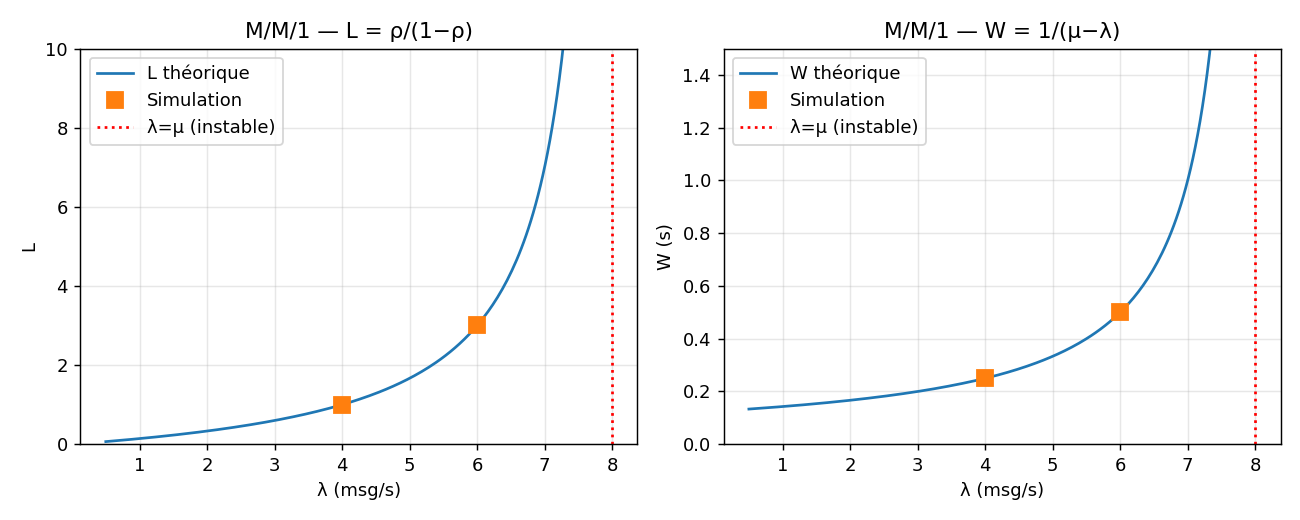
\includegraphics[width=0.92\textwidth]{figures/mm1_LW_lambda.png}
\caption{M/M/1 : les points simulés ($\lambda=4,6$) tombent pile sur les courbes
théoriques $L=\rho/(1-\rho)$ et $W=1/(\mu-\lambda)$, qui divergent en
$\lambda=\mu=8$.}
\label{fig:mm1lw}
\end{figure}

\begin{figure}[h]
\centering
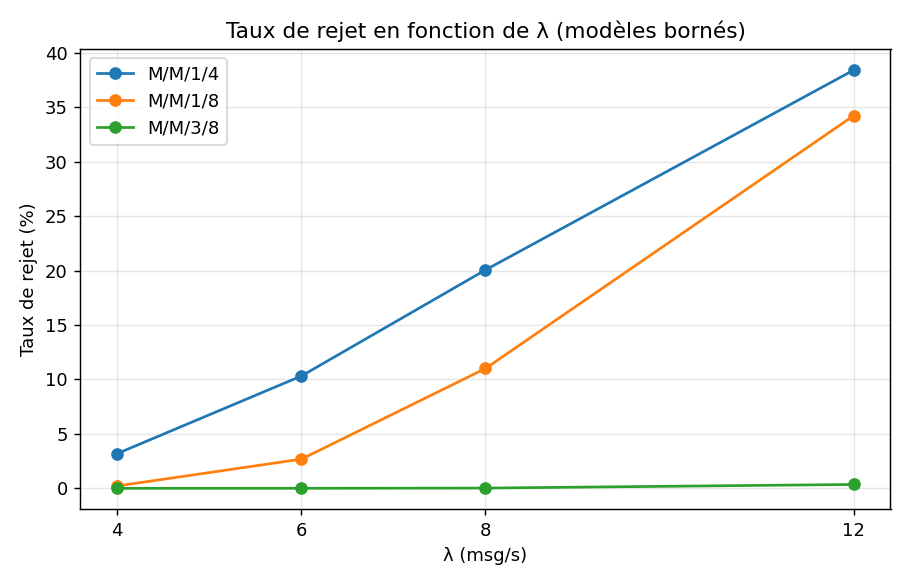
\includegraphics[width=0.7\textwidth]{figures/taux_rejet.png}
\caption{Taux de rejet en fonction de $\lambda$ pour les modèles bornés. À
$\lambda$ égal : M/M/1/8 rejette moins que M/M/1/4 (file plus grande), et
M/M/3/8 rejette quasiment rien (capacité de traitement triplée).}
\label{fig:rejet}
\end{figure}

\begin{figure}[h]
\centering
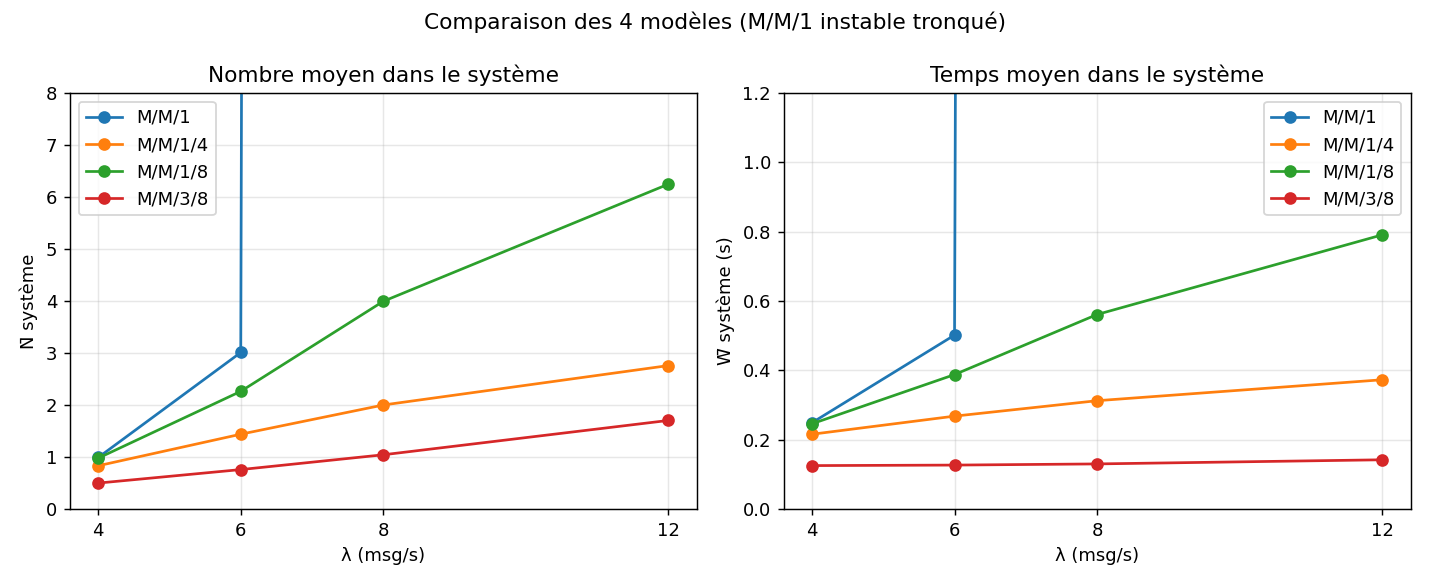
\includegraphics[width=\textwidth]{figures/comparaison_modeles.png}
\caption{Comparaison des quatre modèles (la courbe M/M/1, instable au-delà de
$\lambda=6$, est tronquée). Plus la capacité et le nombre de serveurs
augmentent, plus $\bar N$ et $\bar W$ restent maîtrisés.}
\label{fig:compar}
\end{figure}

\clearpage
% ====================================================================
\section{Analyse des observations}
% ====================================================================
\begin{itemize}
  \item \textbf{M/M/1 et la stabilité.} Pour $\rho<1$ ($\lambda=4,6$) le système
        est stable et les moyennes convergent. Dès $\rho=1$ ($\lambda=8$) la file
        n'est plus stable : on mesure $\bar N \approx 921$ et $\bar W \approx 115$~s,
        et pour $\lambda=12$ des valeurs gigantesques. Ce ne sont pas des valeurs
        \og réelles\fg{} mais le signe d'une file qui grandit sans borne ; la théorie
        donne d'ailleurs $L=W=\infty$.
  \item \textbf{Effet de la borne $K$.} Limiter la capacité stabilise toujours le
        système (même pour $\rho>1$), au prix de pertes. Le taux de rejet croît
        avec $\lambda$ (figure~\ref{fig:rejet}) et, à $\lambda$ donné, une file plus
        grande rejette moins (M/M/1/8 < M/M/1/4).
  \item \textbf{Compromis attente / perte.} Les modèles bornés ont un $\bar W$ plus
        court que M/M/1 (il y a \og moins de monde\fg{} puisqu'on rejette), mais cela
        se paie en messages perdus. C'est le compromis classique délai/perte.
  \item \textbf{Multi-serveurs.} M/M/3/8 est de loin le meilleur : à $\lambda=12$
        il ne perd que $0{,}36\%$ des messages avec $\bar W \approx 0{,}14$~s, là où
        M/M/1/8 en perd $34\%$. Tripler les serveurs divise la charge par serveur
        et la file reste presque toujours vide ($\bar N_{\text{file}}\approx 0{,}2$).
\end{itemize}

% ====================================================================
\section{Comparaison simulation / théorie}
\label{sec:compar}
% ====================================================================
Le tableau~\ref{tab:compar} confronte la simulation à la théorie. Pour M/M/1 on
utilise les formules fermées ; pour les modèles bornés, la formule générale de
naissance--mort M/M/c/K (implémentée dans \texttt{theorie.py}).

\begin{table}[h]
\centering
\small
\begin{tabular}{@{}llrrrrrr@{}}
\toprule
& & \multicolumn{2}{c}{$\bar N_{\text{sys}}$ / $L$} & \multicolumn{2}{c}{$\bar W_{\text{sys}}$ / $W$ (s)} & \multicolumn{2}{c}{Rejet (\%)} \\
\cmidrule(lr){3-4}\cmidrule(lr){5-6}\cmidrule(lr){7-8}
Modèle & $\lambda$ & sim. & théo. & sim. & théo. & sim. & théo. \\
\midrule
M/M/1   & 4  & 0.994 & 1.000 & 0.249 & 0.250 & --- & --- \\
M/M/1   & 6  & 3.011 & 3.000 & 0.502 & 0.500 & --- & --- \\
M/M/1   & 8  & 921.5 & $\infty$ & 115.1 & $\infty$ & --- & --- \\
M/M/1   & 12 & 202246 & $\infty$ & 16925 & $\infty$ & --- & --- \\
\midrule
M/M/1/4 & 4  & 0.835 & 0.839 & 0.216 & 0.217 & 3.20 & 3.23 \\
M/M/1/4 & 6  & 1.441 & 1.444 & 0.268 & 0.269 & 10.32 & 10.37 \\
M/M/1/4 & 8  & 2.002 & 2.000 & 0.313 & 0.313 & 20.06 & 20.00 \\
M/M/1/4 & 12 & 2.759 & 2.758 & 0.373 & 0.373 & 38.41 & 38.39 \\
\midrule
M/M/1/8 & 4  & 0.982 & 0.982 & 0.246 & 0.246 & 0.22 & 0.20 \\
M/M/1/8 & 6  & 2.264 & 2.269 & 0.388 & 0.389 & 2.68 & 2.71 \\
M/M/1/8 & 8  & 3.993 & 4.000 & 0.561 & 0.563 & 11.01 & 11.11 \\
M/M/1/8 & 12 & 6.243 & 6.240 & 0.790 & 0.791 & 34.22 & 34.22 \\
\midrule
M/M/3/8 & 4  & 0.503 & 0.503 & 0.126 & 0.126 & 0.00 & 0.00 \\
M/M/3/8 & 6  & 0.762 & 0.765 & 0.127 & 0.127 & 0.00 & 0.00 \\
M/M/3/8 & 8  & 1.046 & 1.044 & 0.131 & 0.131 & 0.02 & 0.02 \\
M/M/3/8 & 12 & 1.705 & 1.706 & 0.142 & 0.143 & 0.36 & 0.37 \\
\bottomrule
\end{tabular}
\caption{Simulation vs théorie. L'écart est partout inférieur au pour-cent.}
\label{tab:compar}
\end{table}

\noindent\textbf{Commentaires.}
\begin{itemize}
  \item \textbf{M/M/1.} Concordance parfaite sur les cas stables : $0{,}994$ vs $1$ et
        $3{,}011$ vs $3$ pour $\bar N$ ; $0{,}249$ vs $0{,}25$ et $0{,}502$ vs $0{,}5$ pour
        $\bar W$. Les cas $\lambda\ge8$ \og explosent\fg{}, ce qui matérialise bien la
        divergence théorique ($\rho\ge1$).
  \item \textbf{Modèles bornés.} L'accord est tout aussi bon, y compris sur les
        taux de rejet (ex. M/M/1/4 à $\lambda=8$ : $20{,}06\%$ simulé vs $20\%$
        théorique). La formule M/M/c/K reproduit fidèlement M/M/3/8.
  \item \textbf{Loi de Little.} Le contrôle interne $L=\lambda_{\text{eff}}\,W$ est
        vérifié sur tous les runs : la colonne \texttt{little\_L} de
        \texttt{results/resultats.csv} coïncide avec $\bar N_{\text{sys}}$ (ex. M/M/1
        $\lambda=6$ : $3{,}011=3{,}011$). C'est une validation indépendante des
        mesures de temps et de nombre.
\end{itemize}

% ====================================================================
\section{Conclusion}
% ====================================================================
Le simulateur à événements discrets a été implémenté en respectant
l'architecture demandée (une classe par fichier, scheduler sans \texttt{sort()},
trace au bon format) et validé classe par classe. Les quatre modèles donnent des
résultats qui collent à la théorie à mieux qu'un pour-cent, et la loi de Little
est vérifiée partout : le simulateur est correct.

Sur le fond, l'étude illustre les enseignements attendus : M/M/1 devient instable
dès $\rho\ge1$ ; borner la capacité stabilise le système mais introduit des
pertes ; et augmenter le nombre de serveurs (M/M/3/8) est la solution la plus
efficace, avec un temps d'attente faible et presque aucun rejet même en forte
charge.

\end{document}
